\documentclass[border=0.8ex,svgnames,tikz]{standalone}
\usepackage{amsmath,mathtools}
\usepackage{fontspec}
\setmainfont{Source Serif 4}
\setsansfont{Source Sans 3}
\setmonofont{Source Code Pro}
\usepackage{ifthen}
\usetikzlibrary{chains,shapes.multipart,calc}
\makeatletter
\let\widthof=\pgfmath@calc@widthof%
\let\heightof=\pgfmath@calc@heightof%
\let\depthof=\pgfmath@calc@depthof%
\makeatother
\begin{document}
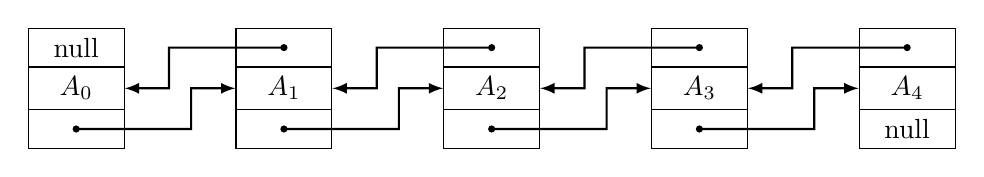
\begin{tikzpicture}
  \begin{scope}[
    every node/.style={
      draw,
      on chain,
      text centered,
      text width=2.8em,
      rectangle split,
      rectangle split parts=3,
      rectangle split every empty part={},
      rectangle split part align={center,center,center},
      rectangle split empty part width=\widthof{null},
      rectangle split empty part height=\heightof{null},
      rectangle split empty part depth=\depthof{null},
    },
    node distance=4em,
    start chain,
    ]
    \foreach \i in {0,...,4}{
      \node(a\i){
        \nodepart{one}\ifthenelse{\i=0}{null}{\phantom{null}}
        \nodepart{two}\(A_{\i}\)
        \nodepart{three}\ifthenelse{\i=4}{null}{\phantom{null}}
      };
    };
  \end{scope}
  \begin{scope}[every path/.style={draw,thick,>=latex}]
    \foreach \i in {0,...,3}{
      \pgfmathtruncatemacro{\x}{\i+1};
      \coordinate(a\x-center) at (a\x.one west-|a\x.one south);
      \coordinate(a\i-prev) at ($(a\x.one west)!0.6!(a\i.one east)$);
      \path[->] (a\x-center) -- (a\i-prev) |- (a\i.two east);
      \fill (a\x-center) circle (0.2ex);
      \coordinate(a\i-center) at (a\i.three west-|a\i.three south);
      \coordinate(a\i-next) at ($(a\i.three east)!0.6!(a\x.three west)$);
      \path[->] (a\i-center) -- (a\i-next) |- (a\x.two west);
      \fill (a\i-center) circle (0.2ex);
    };
  \end{scope}
\end{tikzpicture}
\end{document}
